\chapter{Resultados e Discussões} \label{cap::resultados}



% -.~.-.~.-.~.-.~.-.~.-.~.-.~.-.~.-.~.-.~.-.~.-
\section{Resultados de simulação} \label{sec::resultados}

Os resultados das simulações de cada tarefa proposta são apresentados a seguir
para os seguintes casos de base:
%
\begin{enumerate*}[label=\emph{\roman*})]
	\item base rígida;
	\item base de testes;
	\item base modular PRP;
	\item base telescópica PRPP.
\end{enumerate*}
%

Em todos os casos são avaliados os erros de posicionamento, velocidade e
orientação da ferramenta, ao longo de toda a tarefa. Na
seção~\ref{sec::comparacao} são comparados os resultados para as diferentes
bases.

\subsection{Base rígida} \label{sec::res_rigida}

Seguem os resultados do modelo de base rígida que utiliza o modelo MBS --
Robô.
A Figura~\ref{fig::anim3D_base_rig} apresenta o resultado da simulação no ambiente
3D de cada tarefa.

\begin{figure}[h]
    \centering
    \begin{subfigure}[b]{0.45\textwidth}
        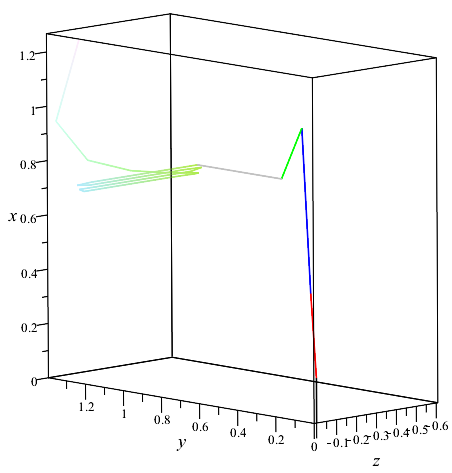
\includegraphics[width=\textwidth]{figs/t1_anima3D_base_rig}
        \caption{Tarefa 1}
        \label{fig::t1_anima3D_base_rig}
    \end{subfigure}
    \quad %add desired spacing between images, e. g. ~, \quad, \qquad, \hfill
    % etc.
      %(or a blank line to force the subfigure onto a new line)
    \begin{subfigure}[b]{0.40\textwidth}
        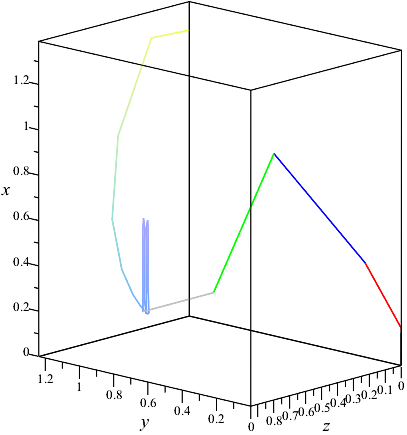
\includegraphics[width=\textwidth]{figs/t2_anima3D_base_rig}
        \caption{Tarefa 2}
        \label{fig::t2_anima3D_base_rig}
    \end{subfigure}
    \caption{Resultado no ambiente 3D das simulações para base rígida}
    \label{fig::anim3D_base_rig}
\end{figure}

Estes resultados representam uma referência para posterior comparação com os
resultados obtidos para o modelo MBS acoplado.


\subsubsection{Posição da ferramenta}

Os resultados de simulação da posição da ponta da ferramenta para Tarefa 1 são
apresentados a seguir. A Figuras~\ref{fig::t1_posf_base_rig} fornece o valor de
cada coordenada $x, y, z$ no referencial inercial (linha cheia) e também o valor
de referência (linha tracejada), fornecido pela cinemática inversa. A
Figura~\ref{fig::t1_posf_base_rig} fornece o erro de posição, ou seja, a
diferença entre o valor de referência dado pela cinemática inversa e o efetivo,
de cada coordenada, assim como o erro absoluto (linha tracejada).

\begin{figure}[h!]
	\centering 
 	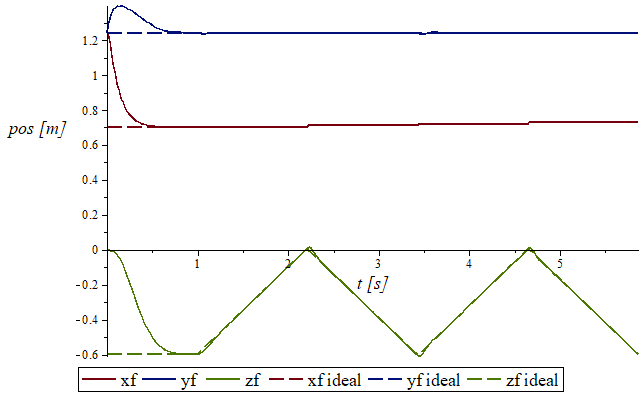
\includegraphics[width=0.80\textwidth]{figs/t1_posf_base_rig}
 	\caption{Posições das coordenadas da ferramenta para base rígida -- Tarefa 1}
 	\label{fig::t1_posf_base_rig}
\end{figure}

\begin{figure}[h!]
	\centering 
 	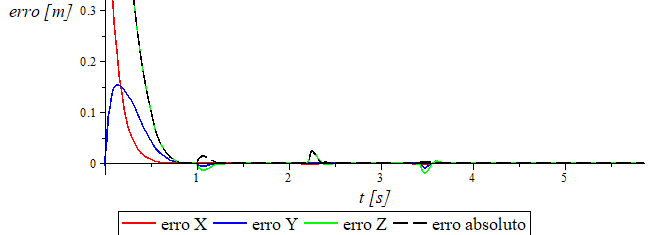
\includegraphics[width=0.80\textwidth]{figs/t1_erroposf_base_rig}
 	\caption{Erro de posição da ferramenta para base rígida -- Tarefa 1}
 	\label{fig::t1_erroposf_base_rig}
\end{figure}

Da mesma forma, apresenta-se os resultados de simulação da posição da ponta da
ferramenta para a Tarefa 2. A Figura~\ref{fig::t2_posf_base_rig} fornece as
posições efetiva (linhas cheias) e ideal (linhas tracejadas). E a
Figura~\ref{fig::t2_erroposf_base_rig} o erro de cada coordenada, com respeito
ao referencial inercial.

\begin{figure}[h!]
	\centering 
 	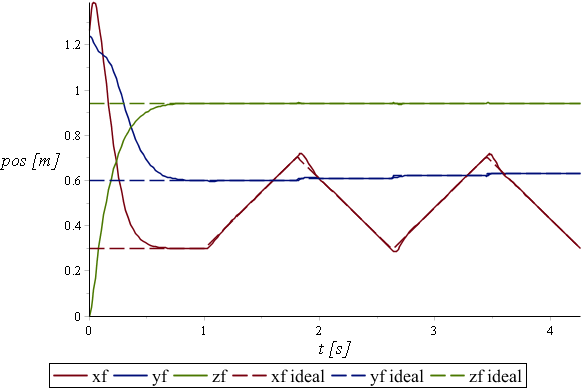
\includegraphics[width=0.80\textwidth]{figs/t2_posf_base_rig}
 	\caption{Posições das coordenadas da ferramenta para base rígida -- Tarefa 2}
 	\label{fig::t2_posf_base_rig}
\end{figure}

\begin{figure}[h!]
	\centering 
 	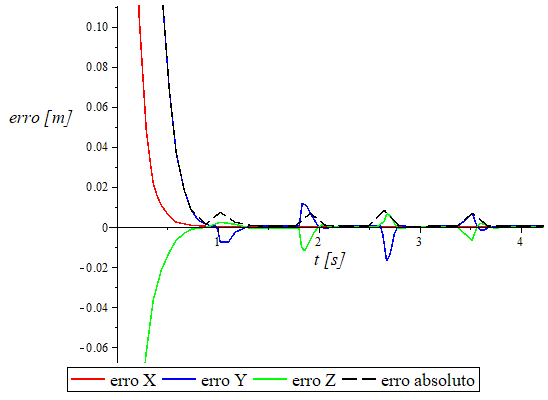
\includegraphics[width=0.80\textwidth]{figs/t2_erroposf_base_rig}
 	\caption{Erro de posição da ferramenta para base rígida -- Tarefa 2}
 	\label{fig::t2_erroposf_base_rig}
\end{figure}


\subsubsection{Velocidade da ferramenta}

São apresentados os gráficos da velocidade da ponta da ferramenta (linhas
cheias) e as velocidades de referência dadas pela cinemática inversa (linhas
tracejadas), na Figura~\ref{fig::t1_velf_base_rig} para a Tarefa 1 e na
Figura~\ref{fig::t1_errovelf_base_rig} os erros em relação a velocidade de
referência, no referencial inercial.

\begin{figure}[h!]
	\centering 
 	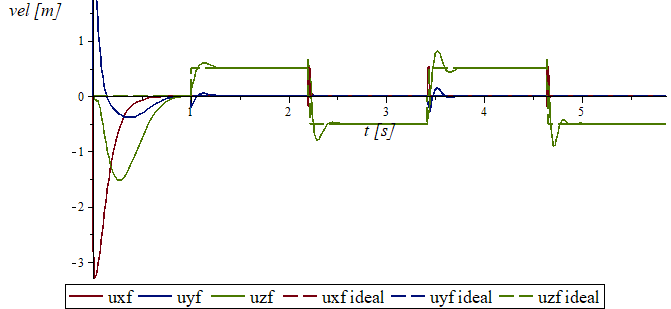
\includegraphics[width=0.80\textwidth]{figs/t1_velf_base_rig}
 	\caption{Velocidades das coordenadas da ferramenta para base rígida -- Tarefa 1}
 	\label{fig::t1_velf_base_rig}
\end{figure}

\begin{figure}[h!]
	\centering 
 	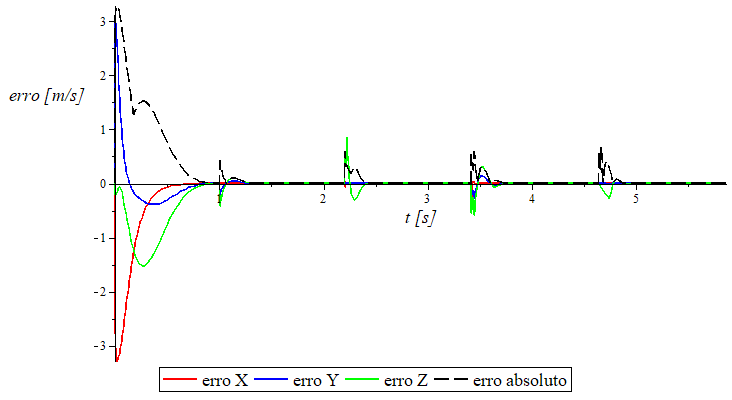
\includegraphics[width=0.80\textwidth]{figs/t1_errovelf_base_rig}
 	\caption{Erro de velocidade da ferramenta para base rígida --
 	Tarefa 1}
 	\label{fig::t1_errovelf_base_rig}
\end{figure}

A seguir, apresenta-se os resultados de simulação da velocidade da ponta da
ferramenta para a Tarefa 2.
A Figura~\ref{fig::t2_posf_base_rig} fornece as velocidades efetivas (linhas
cheias) e ideais (linhas tracejadas). A Figura~\ref{fig::t2_erroposf_base_rig} o
erro de cada coordenada, com respeito ao referencial inercial.

\begin{figure}[h!]
	\centering 
 	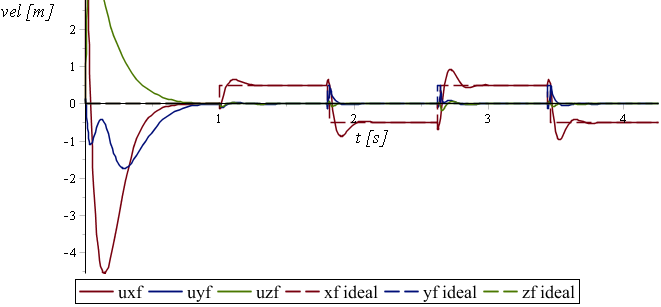
\includegraphics[width=0.80\textwidth]{figs/t2_velf_base_rig}
 	\caption{Velocidades das coordenadas da ferramenta para base rígida -- Tarefa
 	2}
 	\label{fig::t2_velf_base_rig}
\end{figure}

\begin{figure}[h!]
	\centering 
 	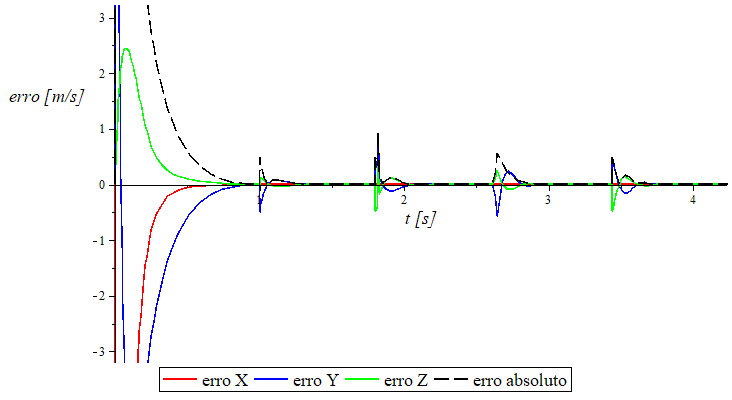
\includegraphics[width=0.80\textwidth]{figs/t2_errovelf_base_rig}
 	\caption{Erro de velocidade da ferramenta para base rígida -- Tarefa 2}
 	\label{fig::t2_errovelf_base_rig}
\end{figure}

\subsubsection{Orientação da ferramenta}

O erro de orientação da ferramenta é resultado da matriz de rotação entre o
referencial inercial e a orientação do pulso, em função dos ângulos de Euler, em
relação a orientação desejada. Faz-se uma transformação da matriz de rotação em
eixo e ângulo, de acordo com as equações~\ref{eq::ang_erro} e
\ref{eq::eixo_erro}.

A Figura~\ref{fig::t1_erroori_base_rig} apresenta o erro de orientação,
representado pelo ângulo $\theta$, para a Tarefa 1. A
Figura~\ref{fig::t2_erroori_base_rig} apresenta o erro de orientação na Tarefa 2.

\begin{figure}[h!]
	\centering 
 	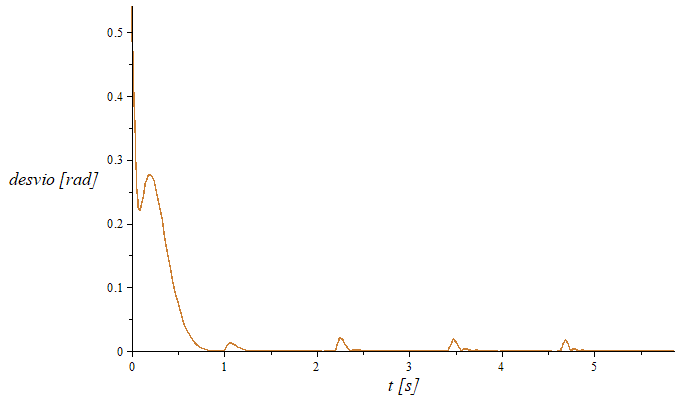
\includegraphics[width=0.80\textwidth]{figs/t1_erroori_base_rig}
 	\caption{Erro de orientação da ferramenta para base rígida -- Tarefa
 	1}
 	\label{fig::t1_erroori_base_rig}
\end{figure}



\begin{figure}[h!]
	\centering 
 	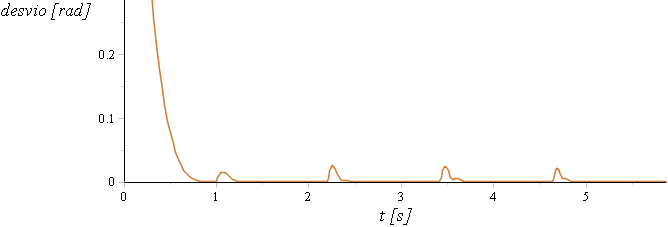
\includegraphics[width=0.80\textwidth]{figs/t2_erroori_base_rig}
 	\caption{Erro de orientação da ferramenta para base rígida -- Tarefa
 	2}
 	\label{fig::t2_erroori_base_rig}
\end{figure}

\subsubsection{Erros máximos - Base rígida}

A Tabela~\ref{tab::erros_base_rig} resume os erros máximos de posição,
velocidade e orientação encontrados em cada tarefa. Os erros de posição
são dados nas 3 coordenadas cartesianas do referencial inercial; o erro
de velocidade é fornecido na direção tangente da trajetória; e o erro de
orientação é dado como um ângulo $\theta$ na direção do eixo $\omega$.

\begin{table}[h!]
\centering
\caption{Resumo dos erros máximos encontrados -- Base Rígida}
\label{tab::erros_base_rig}
\begin{tabular}{@{}ccccccc@{}}
\toprule
         & \multicolumn{3}{c}{\textbf{Posição $[mm]$}} & \textbf{Velocidade $[m/s]$} & \multicolumn{2}{c}{\textbf{Orientação $[rad]$}} 	\\ \midrule
         & x          & y          & z          & tangente            & $\theta$            & $\omega$         		\\
Tarefa 1 & 1,5        & 9,0        & 20,0       & 0,30                &	0,021				& [0,995,~-0,960,~-0,029]                  	\\
Tarefa 2 & 0,07       & 16,5	   & 11,5       & 0,45                & 0,032				& [0,999,~0,002,~0,046] \\ \bottomrule
\end{tabular}
\end{table}


\subsection{Base de testes} \label{sec::res_testes}

\subsubsection{Posição da ferramenta}

\subsubsection{Velocidade da ferramenta}

\subsubsection{Orientação da ferramenta}

\subsection{Base modular PRP} \label{sec::res_prp}

\subsubsection{Posição da ferramenta}

\subsubsection{Velocidade da ferramenta}

\subsubsection{Orientação da ferramenta}

\subsection{Base telescópica PRPP} \label{sec::res_prpp}

\subsubsection{Posição da ferramenta}

\subsubsection{Velocidade da ferramenta}

\subsubsection{Orientação da ferramenta}


% -.~.-.~.-.~.-.~.-.~.-.~.-.~.-.~.-.~.-.~.-.~.-
\section{Comparação dos resultados} \label{sec::comparacao}


% -.~.-.~.-.~.-.~.-.~.-.~.-.~.-.~.-.~.-.~.-.~.-
\section{Possíveis soluções} \label{sec::solucoes}

% if we have a proper knowledge about the dynamics of the system including the
% base motion dynamics, we can develop sophisticated control methods.
% (Artigo: Moving base robotics and reaction management control)
